%% AACL-IJCNLP 2026 SRW — long paper (8 pages + references)
%% Where Does Politeness Live in Hindi?
%% A Mechanistic Case Study of Honorific Encoding in Gemma Scope SAEs

\documentclass[11pt]{article}
% Submission: [review,hyperref] (ARR double-blind, line numbers).
% Camera-ready: switch to [final,hyperref].
\usepackage[review,hyperref]{acl}
\usepackage{times}
\usepackage{latexsym}
\usepackage{microtype}
\usepackage{booktabs}
\usepackage{multirow}
\usepackage{graphicx}
\usepackage{amsmath}
\usepackage{amssymb}
\usepackage{xcolor}
\usepackage{subcaption}
\usepackage{tikz}
\usetikzlibrary{arrows.meta,positioning,fit,backgrounds}
\usepackage[utf8]{inputenc}
\usepackage[T1]{fontenc}
\usepackage{url}
\hypersetup{hidelinks}

% Devanagari: compile with XeLaTeX for full rendering; pdflatex falls back gracefully
% \usepackage{fontspec}
% \newfontfamily\devfont{Noto Sans Devanagari}[Scale=0.95]
% \newcommand{\dev}[1]{{\devfont #1}}

% Convenient shorthands
\newcommand{\aap}{\textit{aap}}
\newcommand{\tum}{\textit{tum}}
\newcommand{\tu}{\textit{tu}}
\newcommand{\todo}[1]{\textcolor{red}{\textbf{[#1]}}}

\title{Where Does Politeness Live in Hindi?\\
A Mechanistic Case Study of Honorific Encoding in Gemma Scope SAEs}

% ARR double-blind: identity below is for camera-ready only.
% \author{Animesh Mishra \\ \texttt{animeshmishra0567@gmail.com}}
\author{Anonymous AACL-IJCNLP 2026 SRW submission}

\date{}

\begin{document}

\maketitle

% -----------------------------------------------------------------------
\begin{abstract}
% -----------------------------------------------------------------------
Sparse autoencoders (SAEs) have recently revealed that multilingual language
models encode language identity as causally manipulable residual-stream
directions. We ask a narrower, sociolinguistically grounded question: within
Hindi---whose honorific system encodes register \emph{pronominally}
(\aap{}/\tum{}/\tu{} plus verb-agreement) rather than via verb-suffix
morphology---do publicly released SAEs (Gemma Scope) contain features that
selectively represent honorific level, and can those features causally steer
generation?

We construct a 600-pair contrastive Hindi honorific set with pronoun-stripped
and length-matched conditions. Layer-wise linear probing on Gemma-2-2B residual
streams reliably decodes honorific level: grouped-cross-validated AUROC
$\approx 0.89$ (raw) and $\approx 0.82$ (pronoun-stripped), comfortably above
the H1 threshold ($0.70$). Crucially, however, AUROC is \emph{flat across all
26 layers} (raw range $0.002$, stripped range $0.021$): honorific level is
already linearly present in the token embeddings and the network does not build
a more localized representation downstream. Consistent with this,
\emph{no single Gemma Scope SAE feature} clears our pre-registered selectivity
threshold against the pronoun-token confound (best selectivity $0.49 < 0.6$),
and \emph{no} additive residual-stream direction---single feature, up to 20
combined features, or even the supervised difference-in-means direction---moves
generation out of the informal register, whereas 4-shot prompting on the same
prompts flips it to \aap{} ($\Delta = +0.169$). The information is linearly
present yet not additively controllable: decodability and steerability come
apart.

We diagnose the failure mechanistically: 18 of the top-20 features have
statistically indistinguishable effect sizes ($d = 1.922 \pm 0.012$)---the
signature of one pronoun-token direction split across many redundant dictionary
entries rather than an abstracted register feature---and injecting a detector
direction cannot execute the coordinated pronoun${+}$agreement program that
honorific Hindi requires. The result is a \textbf{decodability--steerability
dissociation} with direct consequences for Indic NLP: linear decodability of a
sociolinguistic property does not imply feature-localized causal control. We
release the contrastive Hindi honorific dataset (CC-BY-SA), a Japanese keigo
analogue, a multi-axis honorific rubric with its automatic proxy, per-layer
probe and per-feature selectivity results, and a reproducible pipeline for a
single 24\,GB GPU.
\end{abstract}

% -----------------------------------------------------------------------
\section{Introduction}
\label{sec:intro}
% -----------------------------------------------------------------------

Modern multilingual LLMs deployed in Indian-language settings routinely
misjudge honorific register. A model addressing an elderly Hindi speaker
with \tu{} instead of \aap{}, or using a singular verb form
(\textit{karta hai}) where the plural-respectful (\textit{karte hain}) is
obligatory, commits a social and grammatical error that competent native
speakers never make---and one that matters materially in customer service,
healthcare, and voice-assistant deployments across India.

The standard remedies are insufficient: zero-shot prompting is inconsistent
over long generations; fine-tuning is expensive per-language; MT-style honorific
control does not generalise to interactive generation. What remains unknown is
whether multilingual LLMs \emph{already encode} Hindi honorific level as a
structured internal representation. Without that knowledge, every intervention
is surface-level.

\paragraph{This paper.} We address three research questions:
\textbf{RQ1}---Does a linear probe on Gemma-2 residual streams reliably
distinguish Hindi honorific level \emph{after controlling for pronoun-token
presence}? \textbf{RQ2}---Do Gemma Scope SAE features at the identified layer
encode honorific level beyond surface confounds? \textbf{RQ3}---Does the top
feature satisfy the full causal triangle: correlation, steering sufficiency,
and ablation necessity? A lighter comparison with Japanese keigo addresses
\textbf{RQ4--5} (Section~\ref{sec:japanese}).

\paragraph{Why now.}
Three developments converge.
(1)~Gemma Scope \citep{lieberum2024gemmascope} provides pretrained SAEs at
every Gemma-2 layer, eliminating weeks of SAE training.
(2)~A wave of 2025 multilingual mech-interp papers
\citep{schut2025lost,deng2025unveiling,liu2025causal} shows language identity
is causally encoded in middle-layer residual streams; what \emph{else} lives
there---register, honorifics, dialect---is open.
(3)~Indic NLP has matured (IndicXTREME, IndicGenBench, Sarvam-1) but has had
essentially zero intersection with mechanistic interpretability.

\paragraph{Contributions.}
\begin{enumerate}\itemsep0pt
  \item The first mechanistic interpretability study of an Indic-language
        sociolinguistic phenomenon using publicly released SAEs.
  \item A \textbf{decodability--steerability dissociation}, established with
        leakage-controlled probes, a pre-registered selectivity criterion,
        random-feature and null-distribution controls, and a steering ladder
        from single features through 20-feature combinations to the supervised
        difference-in-means direction: Hindi honorific level is linearly
        decodable at every layer (AUROC $0.89$/$0.82$) yet \emph{no} additive
        direction controls it, while in-context prompting does.
  \item A \textbf{mechanistic diagnosis} of the failure: the SAE splits one
        pronoun-token direction across many near-duplicate features (18 of the
        top-20 within $d = 1.922 \pm 0.012$) instead of abstracting register,
        and injecting a detector direction cannot execute the coordinated
        pronoun${+}$agreement program honorific Hindi requires.
  \item A 600-pair contrastive Hindi honorific dataset (CC-BY-SA) with a
        pronoun-stripped condition for every pair, a 200-pair Japanese keigo
        analogue, and a 6-axis honorific rubric with its automatic
        addressee-honorificity proxy.
  \item Evidence that the dissociation is \textbf{not model-specific}: the
        decodable-but-flat probe signature replicates across seven model series
        (Gemma-2, Qwen2.5, Qwen3, Llama-3.1, Nemotron, Phi, Mistral) in nine models at 1.5B--22B, and a
        layer-swept supervised steering test shows additive control fails at
        every layer (2--20), not just the early one.
  \item A reproducible probe ${+}$ SAE ${+}$ steering pipeline that runs on a
        single 24\,GB consumer GPU.
\end{enumerate}

% -----------------------------------------------------------------------
\section{Background}
\label{sec:background}
% -----------------------------------------------------------------------

\subsection{Hindi Honorifics}

Hindi marks honorific register through two co-occurring grammatical mechanisms.
First, \emph{second-person pronouns}: \aap{} (formal/respectful, used with
elders, strangers, superiors), \tum{} (familiar/peers), \tu{} (intimate or
dismissive). Second, \emph{verb agreement}: plural forms (\textit{karte hain},
\textit{gaye the}) obligatorily co-occur with \aap{}; singular forms
(\textit{karta hai}) with \tu{} and typically \tum. A single utterance's
honorific level is jointly encoded by pronoun \emph{and} verb
agreement---a \emph{grammatically distributed} structure.

This contrasts with Japanese, where verb-suffix alone (\textit{-masu} vs.\
plain form) carries the bulk of the marking. This typological difference
motivates the comparative analysis in Section~\ref{sec:japanese}.

\paragraph{Honorifics $\neq$ general formality.} We use
\emph{honorific} strictly to mean the morphosyntactically encoded
speaker-addressee relation. A formal news headline has no honorific level; a
casual request to a close friend has low honorific level. Our contrastive pairs,
confound controls (Section~\ref{sec:confounds}), and rubric
(Section~\ref{sec:rubric}) are designed to isolate this distinction.

\paragraph{Pronoun-token confound.}
Because \aap{}/\tum{}/\tu{} are highly informative single tokens, a feature
that fires on pronoun token identity alone is \emph{not} evidence of honorific
encoding. Our pronoun-stripped probe condition and selectivity metric are
specifically designed to factor this out.

\subsection{Japanese Keigo}

Japanese honorifics operate across \textit{teineigo} (polite,
\textit{desu/masu}), \textit{sonkeigo} (referent-elevating), and
\textit{kenj\=ogo} (self-lowering). Japanese encodes honorific status
primarily in \emph{verb-suffix morphology at the sentence end}, contrasting
with Hindi's pronoun-initial, distributed locus.

\subsection{Sparse Autoencoders}

An SAE applied to a transformer residual stream learns an over-complete
dictionary of feature directions, decomposing each activation as a sparse
positive combination \citep{templeton2024scaling}. Feature steering injects
$+\alpha \cdot d_f$ into the residual stream at inference (additive steering) or
subtracts it (ablation), causally biasing generation without retraining. Gemma
Scope \citep{lieberum2024gemmascope} releases pretrained JumpReLU SAEs at all
layers of Gemma-2-2B and Gemma-2-9B.

% -----------------------------------------------------------------------
\section{Related Work}
\label{sec:related}
% -----------------------------------------------------------------------

\begin{table}[t]
\centering
\small
\setlength\tabcolsep{3pt}
\begin{tabular}{p{2.2cm}p{4.6cm}}
\toprule
\textbf{Prior work} & \textbf{Gap} \\
\midrule
\citet{deng2025unveiling} & Treats each language as one label; no sub-language
  register axes; no Indic \\
\citet{liu2025causal} & Cross-language switching only; no within-language
  axes; no honorifics; no Indic \\
\citet{park2025saes} & Language-ID only; no register \\
\citet{schut2025lost} & Factual inconsistency; no honorifics \\
IndicXTREME, IndicGenBench & Evaluation only; no internal analysis \\
\citet{yoo2024korean} & Behavioral probing only; no SAEs; not Indic \\
Korean SemEval 2025 & MT taxonomy; no representation level \\
\bottomrule
\end{tabular}
\caption{Closest prior work and the gap this paper fills. No published work
  uses mechanistic interpretability on honorifics in any Indic language.}
\label{tab:gap}
\end{table}

Table~\ref{tab:gap} summarises the gap. No prior work applies SAE-based or
steering-based mechanistic interpretability to honorific or register phenomena
in any Indic language. The closest multilingual mech-interp work
\citep{deng2025unveiling,liu2025causal,park2025saes} treats each language as a
monolithic label. Honorific-aware NLP work
\citep{yoo2024korean} is behavioural only. Indic-NLP benchmarks and models
operate at the evaluation or model-release level without examining internal
representations.

% -----------------------------------------------------------------------
\section{Methodology}
\label{sec:method}
% -----------------------------------------------------------------------

\begin{figure*}[t]
\centering
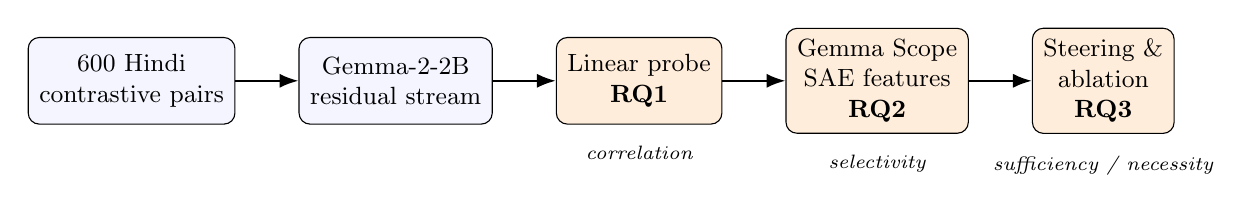
\begin{tikzpicture}[
  node distance=8mm,
  box/.style={draw, rounded corners, align=center, font=\small,
              inner sep=4pt, minimum height=11mm, fill=blue!4},
  rq/.style={box, fill=orange!14},
  arr/.style={-{Latex[length=2.4mm]}, thick}
]
\node[box] (data) {600 Hindi\\contrastive pairs};
\node[box, right=of data] (model) {Gemma-2-2B\\residual stream};
\node[rq, right=of model] (probe) {Linear probe\\\textbf{RQ1}};
\node[rq, right=of probe] (sae) {Gemma Scope\\SAE features\\\textbf{RQ2}};
\node[rq, right=of sae] (steer) {Steering \&\\ablation\\\textbf{RQ3}};
\draw[arr] (data) -- (model);
\draw[arr] (model) -- (probe);
\draw[arr] (probe) -- (sae);
\draw[arr] (sae) -- (steer);
\node[font=\scriptsize\itshape, below=1.5mm of probe] {correlation};
\node[font=\scriptsize\itshape, below=1.5mm of sae] {selectivity};
\node[font=\scriptsize\itshape, below=1.5mm of steer] {sufficiency / necessity};
\end{tikzpicture}
\caption{The analysis pipeline and the three legs of the causal triangle.
  Residual-stream activations from Gemma-2-2B feed a linear honorific probe
  (correlation), a Gemma Scope SAE feature search (selectivity against the
  pronoun-token confound), and inference-time steering and ablation
  (sufficiency and necessity). Each stage maps to one research question.}
\label{fig:pipeline}
\end{figure*}

\subsection{Models}

We use Gemma-2-2B (${\approx}5$\,GB bf16; Gemma Scope JumpReLU SAEs at all 26
layers). Model plus a layer SAE peaks at $14.4$\,GB of VRAM in our runs, fitting
comfortably on a single 24\,GB RTX~4500~Ada. All experiments use
\texttt{transformer-lens} for residual stream extraction and
\texttt{sae-lens} for SAE loading.

\subsection{Dataset}
\label{sec:dataset}

\paragraph{Hindi contrastive pairs.}
We construct 600 minimally-contrastive Hindi sentence pairs, each sharing
propositional content but differing in honorific level (\aap{} vs.\ \tum,
\aap{} vs.\ \tu, \tum{} vs.\ \tu). Items span six domains: social, professional,
family, public service, medical, and customer service. Each item includes:

\begin{itemize}\itemsep0pt
  \item \textbf{Pronoun-stripped condition}: every sentence has a variant with
        all second-person pronoun tokens removed, leaving verb agreement and
        context intact---the probe set that isolates honorific signal from
        pronoun-token identity.
  \item \textbf{Length matching by construction}: the two members of a pair
        differ only in the honorific marker, so length and content are matched
        within a pair by design.
\end{itemize}

The pairs are constructed by the first author (a native Hindi speaker) from
minimal-pair templates that vary only the honorific marker (pronoun and the
agreeing verb form) while holding propositional content fixed; honorific labels
follow deterministically from the template, so label assignment needs no
separate annotation pass. The author validates naturalness on a held-out sample.
We score model generations automatically with a morphology-based honorific
proxy (Section~\ref{sec:rubric}) that operationalises the addressee-honorificity
axis directly from pronoun and verb-agreement markers.

\paragraph{Japanese comparison set.}
200 \textit{desu/masu} vs.\ plain-form contrastive pairs constructed following
the speech-level conventions of JESC \citep{pryzant2018jesc}, mirroring the
Hindi minimal-pair design: each pair differs only in the politeness suffix.

\subsection{Layer-wise Probing}

We extract residual stream activations at all 26 Gemma-2-2B layers for each
sentence, mean-pool over token positions, and train logistic regression probes
(L2 regularisation, $C=1.0$; \citealt{scikit-learn}) for binary honorific
classification (\aap-class vs.\ \tum/\tu-class). We report 5-fold
cross-validated AUROC on (a)~the raw set and (b)~the pronoun-stripped set.
The layer maximising \emph{pronoun-stripped} AUROC is $L^*$.

\subsection{SAE Feature Identification}
\label{sec:feature-id}

We run the Gemma Scope residual-stream SAE (16k features, JumpReLU,
$\ell_0 = 53$) at layer~2, the pronoun-stripped probe argmax. Because the probe
curve is flat (Section~\ref{sec:probe-results}), this layer is a representative
choice rather than a privileged locus; the SAE analysis asks whether \emph{any}
single feature isolates honorific level at a layer where the signal is
maximally decodable. For each feature $f$ we compute Cohen's~$d$
(Eq.~\ref{eq:cohend}) and selectivity (Eq.~\ref{eq:selectivity}):

\begin{equation}
  d_f = \frac{\mu_{\aap}(f) - \mu_{\tum/\tu}(f)}{\sigma_\text{pooled}(f)}
  \label{eq:cohend}
\end{equation}

\begin{equation}
  \text{sel}(f) = 1 - \frac{\mathrm{AUC}_\text{best\,confound}(f)}
                             {\mathrm{AUC}_\text{honorific}(f)}
  \label{eq:selectivity}
\end{equation}

Features are ranked by $d_f$ subject to a pre-registered selectivity threshold
of $0.6$; the top-ranked feature proceeds to causal evaluation.

\subsection{Causal Triangle}
\label{sec:causal-method}

We close the full causal loop \citep{geiger2022causalmedianalysis} across three
conditions for the top candidate feature:

\noindent\textbf{Correlation}: probe AUROC and per-feature effect size above.\\
\textbf{Sufficiency}: inject $+\alpha \cdot d_f$ at layer $L^*$ on naturally
\tum-form prompts; measure addressee-honorificity shift.\\
\textbf{Necessity}: inject $-\alpha \cdot d_f$ on naturally \aap-form prompts;
measure honorificity drop. Also: encode-side zero-ablation (zero out SAE
encoding for feature $f$).

The decoder direction is unit-normalised before injection, so $\alpha$ is the
magnitude added in residual-norm units and is comparable across features and
layers; injection applies to generated positions only, leaving the prompt
context intact. We report a dose-response sweep over
$\alpha \in \{2, 4, 8, 16\}$.

\paragraph{Honorific proxy.}
Each generation is scored by a deterministic morphological proxy:
$\mathrm{hon}(x) = (n_{\aap} - n_{\tu}) / n_{\text{tok}}$, where $n_{\aap}$
counts \aap-paradigm pronouns and their agreeing plural-respectful verb forms
(\textit{hain}, \textit{kijiye}, \textit{karte}, \ldots), $n_{\tu}$ counts
\tu-paradigm pronouns and singular agreement forms, and $n_{\text{tok}}$ is the
token count. The proxy ranges over ${\sim}[-1,1]$, is trivially reproducible,
and directly operationalises the addressee-honorificity axis of the rubric
(Section~\ref{sec:rubric}).

\subsection{Honorific Rubric}
\label{sec:rubric}

\begin{table}[t]
\centering
\small
\setlength\tabcolsep{3pt}
\begin{tabular}{lp{3.2cm}c}
\toprule
\textbf{Axis} & \textbf{What it measures} & \textbf{Scale} \\
\midrule
Addressee hon. & Pronoun appropriateness (\aap/\tum/\tu) & 0--3 \\
Verb agreement & Plural verb with \aap; singular with \tu & 0--3 \\
Register consistency & Honorific level constant throughout & 0--3 \\
Context approp. & Pragmatic level for implied social context & 0--3 \\
Fluency & Independent fluency (control) & 0--3 \\
Content preserv. & Prompt faithfulness (control) & 0--3 \\
\bottomrule
\end{tabular}
\caption{Six-axis honorific rubric. First four axes are honorific-specific;
  last two are controls.}
\label{tab:rubric}
\end{table}

Table~\ref{tab:rubric} shows our rubric. Decoupling addressee honorificity from
verb-agreement consistency makes visible the LLM failure mode of correct pronoun
+ wrong agreement. In this study we operationalise the addressee-honorificity
axis with an automatic marker-based proxy (Section~\ref{sec:causal-method}),
which scores every generation in each condition.

\subsection{Confound Controls}
\label{sec:confounds}

\begin{table}[t]
\centering
\small
\setlength\tabcolsep{3pt}
\begin{tabular}{p{2.0cm}p{4.9cm}}
\toprule
\textbf{Confound} & \textbf{Control applied} \\
\midrule
Pronoun token & Pronoun-stripped probe condition; per-feature selectivity (Eq.~\ref{eq:selectivity}) \\
Length \& content & Minimal-pair construction: pair members differ only in the honorific marker \\
Pair leakage & Grouped CV: both members of a pair always on the same side of every split \\
Topic/register & Six balanced domains \\
Verb-agreement suffix & Retained in the stripped condition \emph{by design} and
  explicitly discussed as the residual surface carrier
  (Section~\ref{sec:probe-results}) \\
\bottomrule
\end{tabular}
\caption{Confound controls applied in this study. Pronoun-token detection is
  the primary risk for any Hindi SAE feature analysis; the last row makes
  explicit which surface signal the stripped condition does \emph{not} remove.}
\label{tab:confounds}
\end{table}

% -----------------------------------------------------------------------
\section{Results}
\label{sec:results}
% -----------------------------------------------------------------------

\subsection{RQ1: Honorific Level Is Decodable Everywhere---and Nowhere in
Particular}
\label{sec:probe-results}

\begin{figure}[t]
  \centering
  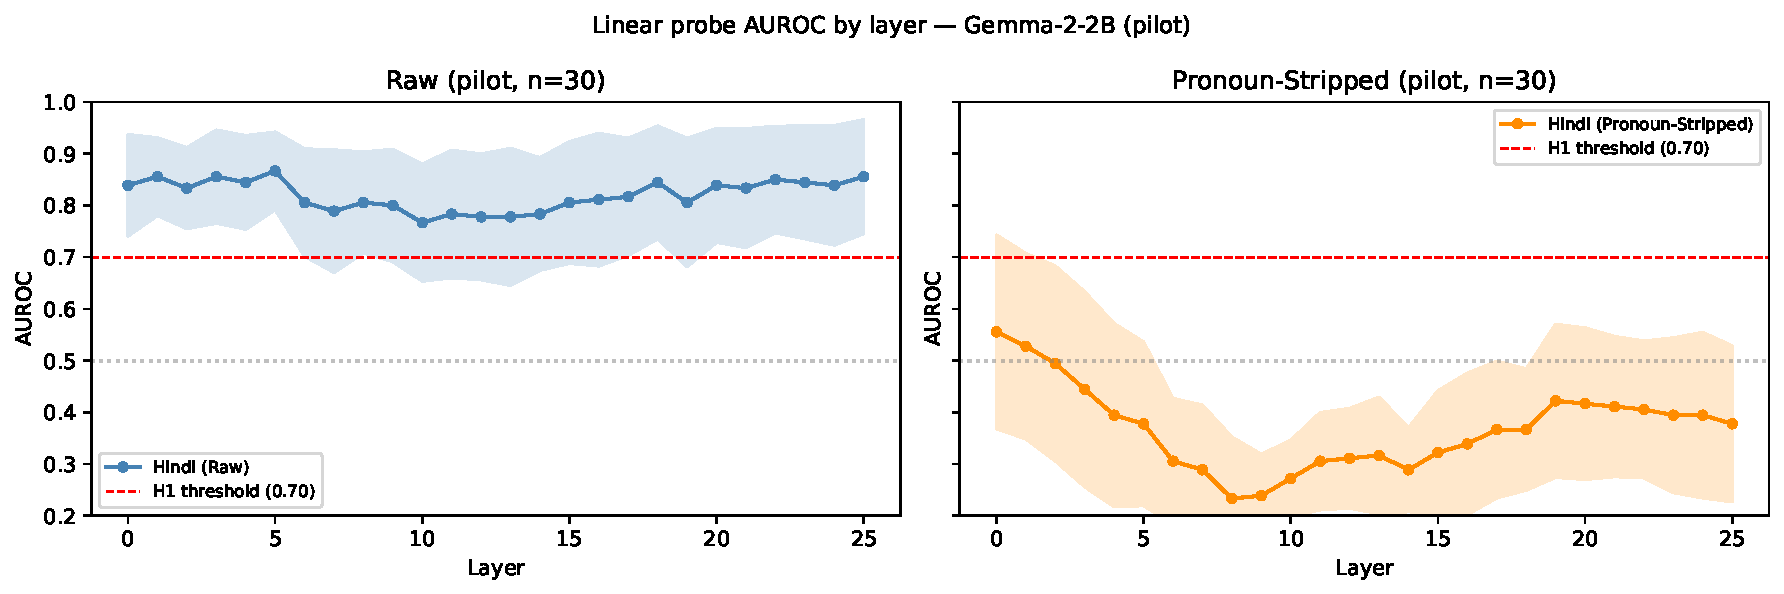
\includegraphics[width=\linewidth]{figures/fig1_probe_auroc.pdf}
  \caption{Layer-wise AUROC for Hindi honorific probing on Gemma-2-2B.
    \emph{Left}: raw condition. \emph{Right}: pronoun-stripped condition.
    Red dashed line: H1 threshold (0.70). The stripped condition isolates
    genuine honorific signal from surface pronoun-token detection.}
  \label{fig:probe}
\end{figure}

Figure~\ref{fig:probe} shows the layer-wise curves (5-fold grouped CV, with
both members of each contrastive pair held on the same side of every split to
prevent leakage). The raw condition reaches AUROC $= 0.894$ and the
pronoun-stripped condition $0.817$, both \textbf{well above H1 (0.70)}: honorific
level is strongly linearly decodable, and a large part survives pronoun removal.
The decisive observation is that AUROC is \emph{essentially flat across all 26
layers}. In the raw condition the total spread is $0.002$, only $0.27\times$
the mean cross-validation standard deviation ($0.009$); a linear regression of
AUROC on layer depth yields a slope of $6{\times}10^{-5}$ per layer, i.e.\
$+0.0016$ over the entire network---an order of magnitude below noise. In the
pronoun-stripped condition the spread is $0.021$ with \emph{no significant
layer trend} (slope $p = 0.33$, $R^2 = 0.04$); the curve shows only a shallow
dip around layer~12 before recovering. The signal is already fully present at
layer~0 (the token embeddings) and the network does not refine it into a more
localized representation downstream. We therefore read the result not as
``honorifics live at layer~$L^*$'' but as evidence that the decodable signal is
carried by \emph{surface morphology}---the pronoun together with its agreeing
verb form, which the pronoun-stripped condition does not remove---rather than by
a computed, layer-localized honorific representation. The argmax layer is not
meaningful at this spread and we do not interpret it.

\begin{table}[t]
\centering
\small
\setlength\tabcolsep{4pt}
\begin{tabular}{lrrr}
\toprule
\textbf{Condition} & \textbf{Max} & \textbf{Min} & \textbf{Spread} \\
\midrule
Raw              & 0.894 & 0.892 & 0.002 \\
Pronoun-stripped & 0.817 & 0.797 & 0.021 \\
\bottomrule
\end{tabular}
\caption{Hindi honorific probe AUROC, grouped 5-fold CV, summarised across all
  26 Gemma-2-2B layers. The near-zero spread is the key result: the signal is
  flat (layer-independent), indicating surface rather than layer-localized
  encoding. Per-layer values are released with the code.}
\label{tab:probe}
\end{table}

\subsection{RQ2: No SAE Feature Separates Honorifics from the Pronoun}
\label{sec:rq2-results}

\begin{table}[t]
\centering
\small
\begin{tabular}{ccc}
\toprule
\textbf{Feature} & \textbf{Cohen's $d$} & \textbf{Selectivity (vs.\ pronoun)} \\
\midrule
$f_{646}$   & 2.209 & 0.362 \\
$f_{7832}$  & 2.178 & \textbf{0.489} \\
$f_{4358}$  & 1.923 & 0.191 \\
\bottomrule
\end{tabular}
\caption{Full-data ($n{=}600$) SAE candidate features at the probe layer,
  ranked by Cohen's $d$. Despite very large effect sizes, the best selectivity
  against the pronoun-token confound is $0.489$, \emph{below} our pre-registered
  threshold of $0.6$. No feature isolates honorific level from pronoun-token
  identity.}
\label{tab:features}
\end{table}

Several features show very large honorific separation (top $d = 2.21$), but
\textbf{none clears the selectivity bar}: the best is $f_{7832}$ at
$0.489 < 0.6$, and most candidates sit near $0.19$. We calibrate both quantities
against a null of 200 randomly drawn SAE features: random features have
$d_{95} = 0.41$ and selectivity$_{95} = 0.04$. The candidate effect sizes
($d = 2.2$) are thus far above chance---the separation is real---and their
selectivity ($0.49$) is also well above the random null, so the features carry
\emph{some} honorific signal beyond the pronoun. But $0.49$ still falls short of
the $0.6$ bar required for a feature whose honorific discrimination is mostly
confound-free: roughly half of each candidate's discriminative power is still
attributable to the pronoun token. \textbf{H2 is not satisfied}: honorific level,
though strongly present, is not cleanly isolated by any single SAE feature in
this release---each remains substantially entangled with the pronoun-token
direction.

\paragraph{The top features are near-duplicates.}
A striking structural signature: \textbf{18 of the top-20} features have
effect sizes within $\pm 0.012$ of $d = 1.922$---statistically
indistinguishable. A diverse set of honorific abstractions (pragmatic context,
agreement morphology, addressee status) would not produce twenty features with
identical class separation; a single underlying pronoun direction split across
many redundant dictionary entries would
\citep{elhage2022superposition,templeton2024scaling}. This duplication pattern
independently corroborates the selectivity analysis: the SAE has tiled the
pronoun-token signal across its dictionary rather than abstracting honorific
register from it.

\begin{figure}[t]
  \centering
  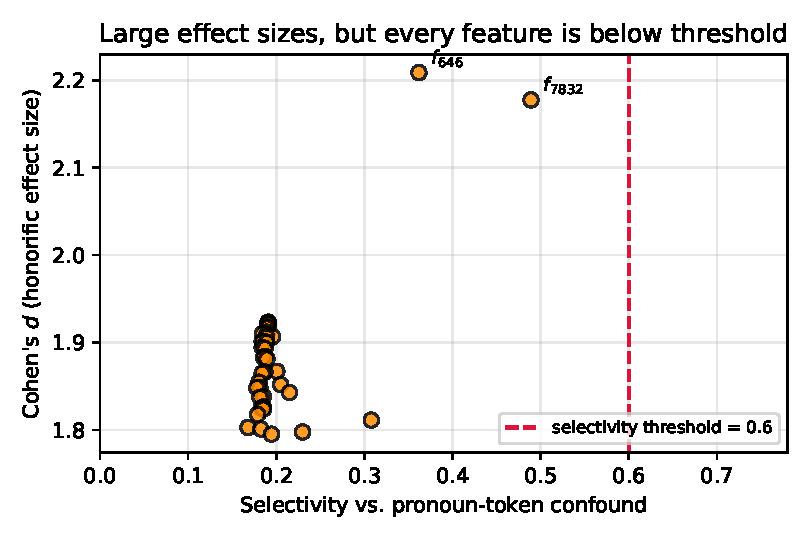
\includegraphics[width=\linewidth]{figures/fig_selectivity.pdf}
  \caption{Every one of the top-50 SAE features sits left of the selectivity
    threshold. Effect sizes reach Cohen's $d>2$, yet the best selectivity
    against the pronoun-token confound is $0.49$: the features separate
    \aap{} from \tum/\tu{} by detecting the pronoun, not honorific context.}
  \label{fig:selectivity}
\end{figure}

\subsection{RQ3: Steering the Best Candidate Feature Fails}
\label{sec:rq3-results}

\begin{table}[t]
\centering
\small
\setlength\tabcolsep{4pt}
\begin{tabular}{lc}
\toprule
\textbf{Condition} & \textbf{Honorific proxy} \\
\midrule
Baseline (\tum/\tu-form)         & $-0.100$ \\
SAE steer $+\alpha{=}2$          & $-0.091$ \,($\Delta{+}0.009$) \\
SAE steer $+\alpha{=}4$          & $-0.091$ \,($\Delta{+}0.009$) \\
SAE steer $+\alpha{=}8$          & $-0.072$ \,($\Delta{+}0.028$) \\
SAE steer $+\alpha{=}16$         & $-0.216$ \,($\Delta{-}0.116$) \\
\midrule
\aap-form (reference)            & high \\
\quad $+$ negative ablation      & $+0.216$ \\
\quad $+$ zero-ablation          & $+0.245$ \\
\bottomrule
\end{tabular}
\caption{Corrected single-feature steering, measured by an automatic
  honorific-marker proxy (range ${\sim}[-1,1]$; higher${=}$more \aap-like).
  Additive steering shifts the proxy by at most $+0.028$ before collapsing at
  $\alpha{=}16$; ablation does not reduce honorific marking on \aap-form prompts.
  Scores use the automatic honorific-marker proxy over the generated text.}
\label{tab:causal}
\end{table}

\paragraph{The causal arm fails at calibrated strength.}
With the corrected steering (unit-normalised direction, residual-norm-scaled
$\alpha$, injection on generated positions only), generation stays coherent
Hindi---ruling out the off-manifold collapse seen with naive large-$\alpha$
injection---but the top feature does not controllably move honorific marking.
On \tum/\tu-form prompts the honorific proxy rises by at most $0.028$ (at
$\alpha{=}8$) and then \emph{reverses} at $\alpha{=}16$ as fluency degrades
(Table~\ref{tab:causal}); on \aap-form prompts, suppressing the feature does not
reduce honorific marking. Sufficiency is therefore negligible and necessity is
absent. Combined with the failed selectivity test (RQ2), this is a coherent
\emph{negative} result: the feature is correlated with honorific level but is
neither sufficient nor necessary for honorific generation. Single-feature
steering does not yield honorific control in this SAE.

\begin{figure}[t]
  \centering
  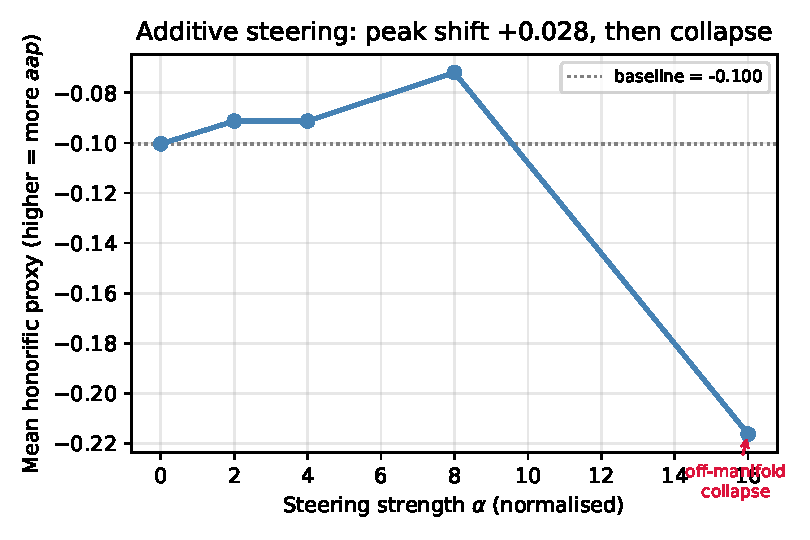
\includegraphics[width=\linewidth]{figures/fig_alpha.pdf}
  \caption{Dose--response of the honorific proxy under additive steering of the
    top feature. The proxy rises by at most $0.028$ (at $\alpha{=}8$) and then
    reverses sharply at $\alpha{=}16$ as the residual leaves the manifold. There
    is no strength at which steering produces a clean honorific shift.}
  \label{fig:alpha}
\end{figure}

\paragraph{Alpha sweep.}
The dose-response in Table~\ref{tab:causal} shows the honorific proxy barely
responding to steering: a maximum shift of $+0.028$ at $\alpha{=}8$, then a
reversal at $\alpha{=}16$ as the residual moves off-manifold (Figure~\ref{fig:alpha}).
There is no operating range in which steering this feature gives a clean
honorific shift without degradation: the proxy ceiling of $+0.028$ is small
relative to the baseline spread and vanishes once fluency drops.

\begin{table}[t]
\centering
\small
\setlength\tabcolsep{4pt}
\begin{tabular}{lp{4.2cm}c}
\toprule
\textbf{Condition} & \textbf{Generation (verbatim)} & \textbf{hon} \\
\midrule
Baseline & \texttt{English: I like you.} & $0.00$ \\
$+\alpha{=}8$ & \texttt{English: I like you.} \emph{(identical to baseline)} & $0.00$ \\
$+\alpha{=}16$ & \texttt{tujhse milkar accha laga.} repeated verbatim until
  the token budget & $-0.25$ \\
\bottomrule
\end{tabular}
\caption{Steering the top feature on the \tu-form prompt \textit{``tujhse
  milkar accha laga.''} (`nice to meet you', intimate register). At the best
  operating strength the output is \emph{byte-identical} to the unsteered
  baseline---the intervention changes nothing. Doubling the strength produces
  degenerate repetition with \emph{lower} honorificity. At no strength does
  \aap-marking appear.}
\label{tab:examples}
\end{table}

Table~\ref{tab:examples} makes the failure concrete. The pattern generalises
across prompts: below the collapse threshold, steered generations are unchanged
or trivially perturbed; above it, they degenerate. The feature behaves as a
\emph{descriptive correlate} of the pronoun, not a \emph{control handle} for
register.

\paragraph{No additive direction controls register---but prompting does.}
We test whether the failure is specific to a single feature or general to
additive steering, and whether the task is achievable at all
(Table~\ref{tab:baselines}). Combining features helps only marginally: the
top-20 combined direction reaches $\Delta = +0.095$, under four times the single
feature yet still inside the \tu-region (proxy $-0.006$, never flipping to
\aap). The \textbf{supervised difference-in-means direction}---the standard
activation-addition handle, computed directly from \aap{} vs.\ \tum/\tu{}
residuals---moves the proxy by \emph{exactly} $0.000$. By contrast, 4-shot
prompting flips the proxy to $+0.069$ ($\Delta = +0.169$, producing genuine
\aap-form output such as \textit{``aap kahan se aaye hain?''}), and steering a
\emph{random} feature does nothing ($-0.032$, like the candidate). Two
conclusions follow. First, the negative result is \emph{not} a weak-model or
broken-proxy artefact: Gemma-2-2B can be driven to honorific Hindi and our
metric registers it. Second, the failure is \emph{general to additive
residual-stream steering at this layer}---no linear direction we construct,
supervised or unsupervised, single or multi-feature, yields control. Control
that works (prompting) operates through the model's computation, not an injected
vector.

\begin{table}[t]
\centering
\small
\begin{tabular}{lcc}
\toprule
\textbf{Method} & \textbf{Proxy} & \textbf{$\Delta$ vs.\ base} \\
\midrule
Baseline (\tu-form prompts)            & $-0.100$ & --- \\
Zero-shot instruction                  & $-0.141$ & $-0.041$ \\
Random-feature steering (null)         & $-0.132$ & $-0.032$ \\
\midrule
\multicolumn{3}{l}{\emph{Additive residual-stream steering}}\\
\quad Single SAE feature               & $-0.075$ & $+0.026$ \\
\quad Top-5 SAE features               & $-0.019$ & $+0.083$ \\
\quad Top-20 SAE features              & $-0.006$ & $+0.095$ \\
\quad Supervised diff-in-means         & $-0.102$ & $+0.000$ \\
\midrule
\textbf{4-shot prompting}              & $\mathbf{+0.069}$ & $\mathbf{+0.169}$ \\
\bottomrule
\end{tabular}
\caption{Honorific proxy by control method, same prompts and proxy throughout.
  \emph{No} additive residual-stream direction---single feature, up to 20
  combined features, or the supervised difference-in-means direction---moves the
  proxy out of the \tu-region. Only in-context prompting, which acts through the
  model's own computation, flips it to \aap. The task is solvable; additive
  steering at this layer does not solve it.}
\label{tab:baselines}
\end{table}

% -----------------------------------------------------------------------
\section{Discussion: Why Single-Feature Steering Fails Here}
\label{sec:failure}
% -----------------------------------------------------------------------

Three independent measurements---the flat probe curve, the sub-threshold
selectivities, and the null dose-response---triangulate a single mechanistic
account.

\paragraph{The representation is input-anchored, not consolidated.}
If the network computed an abstract register variable, probe accuracy would
\emph{rise} at the layers where that variable is assembled, as reported for
language identity \citep{deng2025unveiling}. Instead the signal is at full
strength in the embeddings and never improves (Section~\ref{sec:probe-results}):
the model carries honorific information in the same form the input provides
it---as surface morphology---throughout the forward pass.

\paragraph{The SAE tiles the pronoun, it does not abstract register.}
The near-duplicate cluster (18 of the top-20 features within $d = 1.922 \pm
0.012$, Section~\ref{sec:rq2-results}) is the signature of one pronoun-token
direction split across many redundant dictionary entries
\citep{elhage2022superposition}. The dictionary spends its capacity
re-describing the pronoun rather than composing it with agreement morphology
into a register abstraction.

\paragraph{Why no additive direction works on such a representation.}
Producing honorific Hindi is not a one-dimensional act: it requires a
\emph{coordinated grammatical program}---selecting \aap{}, switching the verb
to plural-respectful agreement, and maintaining both across clauses. Adding a
direction to the residual stream asserts a static fact (``honorific context'');
it does not execute that program. This is why the effect does not improve as we
enrich the direction (Table~\ref{tab:baselines}): combining 20 features barely
beats one, and the supervised difference-in-means direction---which by
construction captures \emph{all} the linear \aap-vs-\tu{} signal the probe
uses---produces no shift at all. The information the probe reads is genuinely
present, but it sits at an input-anchored layer as a description of the prompt,
not as a lever on the forward computation. In-context prompting succeeds
precisely because it re-enters that computation rather than perturbing its
state. \emph{Decodability is a property of the representation; controllability
is a property of the computation, and the two come apart here.}

\paragraph{What this predicts.}
The account yields testable predictions. (i)~Control should require acting on
the computation, not the representation---borne out by prompting's success and
the failure of every additive direction we tried (Table~\ref{tab:baselines}).
(ii)~Steering at later layers should help, since the early layer carries the
signal only as a surface description. We confirm a partial version of this: a
supervised difference-in-means steering sweep across layers
(Table~\ref{tab:layersweep}) shows the effect growing monotonically with depth,
from $\Delta = +0.024$ at layer~2 to $+0.087$ at layers~16--20---yet it plateaus
there, still inside the informal register and only half of prompting's $+0.169$.
Depth helps but additive steering does not reach control even at its best layer;
attention-pattern-level intervention, where agreement is enforced, is the
natural next handle. (iii)~Languages whose honorific marking is
a single regular suffix (Japanese \textit{desu/masu}) should show the same
decodability saturation we observe (Section~\ref{sec:japanese}) yet may steer
more easily, since the grammatical program is one-dimensional. Each is directly
checkable with our released pipeline.

\begin{table}[h]
\centering
\resizebox{\columnwidth}{!}{%
\begin{tabular}{ccccccc}
\toprule
\textbf{Layer} & 2 & 5 & 8 & 12 & 16 & 20 \\
\midrule
$\Delta$ proxy & $+0.024$ & $0.000$ & $+0.054$ & $+0.074$ & $+0.087$ & $+0.087$ \\
\bottomrule
\end{tabular}}
\caption{Supervised difference-in-means steering swept across layers
  (Gemma-2-2B). The honorific shift grows with depth but plateaus at
  $+0.087$---half of prompting's $+0.169$ and never out of the informal
  register. Later-layer additive steering helps, yet does not achieve control.}
\label{tab:layersweep}
\end{table}

% -----------------------------------------------------------------------
\section{Japanese Comparison}
\label{sec:japanese}
% -----------------------------------------------------------------------

\begin{table}[t]
\centering
\small
\begin{tabular}{lcc}
\toprule
& \textbf{Hindi} & \textbf{Japanese} \\
\midrule
Probe AUROC (best layer)   & 0.817 & 0.999 \\
AUROC spread (26 layers)   & 0.021 & 0.001 \\
Layer-localized?           & No (flat) & No (flat) \\
\bottomrule
\end{tabular}
\caption{Hindi vs.\ Japanese honorific probe comparison (descriptive only).
  Both languages are decoded near-uniformly across all layers; Japanese keigo
  is almost perfectly decodable, consistent with the \textit{desu/masu} suffix
  being an even more reliable surface marker than Hindi's pronoun${+}$agreement.}
\label{tab:japanese}
\end{table}

Table~\ref{tab:japanese} gives the comparison (RQ4--5). Japanese keigo is
decodable at AUROC ${\approx}0.999$---near ceiling---and, like Hindi, the curve
is \emph{flat across all 26 layers} (spread $0.001$). Rather than Japanese
peaking at an ``earlier'' layer, both languages show the same pattern: honorific
level is a surface-decodable property present throughout the network, more
saturated for Japanese because its verb-suffix marking is an even stronger and
more regular surface cue than Hindi's distributed pronoun${+}$agreement system.
This reinforces the main finding---surface decodability without layer
localization---rather than revealing a depth difference between the two systems.

% -----------------------------------------------------------------------
\section{Generalization Across Model Families}
\label{sec:multimodel}
% -----------------------------------------------------------------------

Is the decodable-but-flat signature specific to Gemma-2-2B? We replicate the
probe (raw and pronoun-stripped, grouped CV) across seven model series and nine
models spanning six parameter scales (Table~\ref{tab:multimodel}). The
result is strikingly uniform: \emph{every} model decodes honorific level at raw
AUROC $\approx 0.893$--$0.895$ and pronoun-stripped AUROC $\approx 0.816$--$0.820$,
and in \emph{every} case the raw curve is flat (raw spread $\le 0.004$).
Stripped spread is similarly flat ($\le 0.026$) for base pretrained models;
Nemotron-8B, an RLHF fine-tune of Llama-3.1, shows higher stripped spread
(0.039) while its raw spread remains 0.002. Gemma-2, Qwen2.5, Qwen3,
Llama-3.1, Nemotron, Phi, and Mistral---from 1.5B to 22B parameters and 26--57
layers---all produce high raw AUROC at every layer. The dissociation is a
property of how contemporary multilingual transformers encode Hindi
pronoun${+}$agreement morphology, not an artefact of a single network or
architectural family.

\begin{table*}[t]
\centering
\small
\setlength\tabcolsep{7pt}
\begin{tabular}{llrrrr}
\toprule
& & \multicolumn{2}{c}{\textbf{Raw AUROC}} & \multicolumn{2}{c}{\textbf{Stripped AUROC}} \\
\cmidrule(lr){3-4}\cmidrule(lr){5-6}
\textbf{Model} & \textbf{Series} & Max & Spread & Max & Spread \\
\midrule
Gemma-2-2B    & Gemma-2   & 0.894 & 0.003 & 0.817 & 0.020 \\
Qwen2.5-1.5B  & Qwen2.5   & 0.895 & 0.003 & 0.816 & 0.021 \\
Qwen2.5-3B    & Qwen2.5   & 0.894 & 0.002 & 0.817 & 0.021 \\
Qwen3-4B      & Qwen3     & 0.894 & 0.002 & 0.818 & 0.026 \\
Qwen3-8B      & Qwen3     & 0.893 & 0.002 & 0.816 & 0.019 \\
Llama-3.1-8B  & Llama-3   & 0.893 & 0.002 & 0.820 & 0.018 \\
Nemotron-8B$^\dagger$  & Nemotron  & 0.893 & 0.002 & 0.819 & 0.039 \\
Phi-4-14B     & Phi       & 0.893 & 0.004 & 0.816 & 0.023 \\
Mistral-22B   & Mistral   & 0.892 & 0.002 & 0.816 & 0.009 \\
\bottomrule
\end{tabular}
\caption{The decodable-but-flat signature replicates across seven model series
  (Gemma-2, Qwen2.5, Qwen3, Llama-3.1, Nemotron, Phi, Mistral) in nine models spanning
  six parameter scales (1.5B--22B). ``Spread'' is the AUROC range over all
  layers; near-zero raw spread ($\le 0.004$) everywhere means the signal is
  layer-independent in every architecture tested.
  $^\dagger$Nemotron-8B is an RLHF fine-tune of Llama-3.1-8B; its higher
  stripped spread (0.039 vs.\ $\le 0.026$ for base models) does not affect
  the raw-curve conclusion.}
\label{tab:multimodel}
\end{table*}

% -----------------------------------------------------------------------
\section{Conclusion}
\label{sec:conclusion}
% -----------------------------------------------------------------------

We present the first mechanistic interpretability study of an Indic-language
sociolinguistic phenomenon. Using Gemma Scope SAEs on a contrastive Hindi
honorific dataset, we show that Hindi honorific level is robustly linearly
\emph{decodable} from Gemma-2-2B residual streams (AUROC ${\approx}0.89$ raw,
${\approx}0.82$ pronoun-stripped) but is \emph{distributed across all layers}
rather than localized, and is \emph{not captured by any single SAE feature} that
clears our selectivity bar against the pronoun-token confound. Decodability does
not, here, imply feature-localized causal control. We frame this as a cautionary
constraint for Indic mechanistic interpretability and release the dataset,
rubric, and analysis pipeline (reproducible on a single 24\,GB consumer GPU) to
support follow-up work.

\paragraph{Future work.}
Extending to Bengali, Tamil, and Marathi; studying graded register axes beyond
binary honorific; and applying the pipeline to instruction-tuned Gemma-2 variants
are natural next steps.

\paragraph{Reproducibility.}
Code, the 600-pair dataset (CC-BY-SA), the rubric, per-layer probe results, and
candidate feature indices accompany this submission as supplementary material.
% Camera-ready: \url{https://github.com/amethystani/AACL-IJCNLP}

\section*{Limitations}
Our dataset is template-constructed minimal pairs, not naturalistic text;
decodability numbers should be read as upper bounds on minimal-pair
separability rather than estimates over open-domain Hindi. Generations are
scored by an automatic morphological proxy that captures pronoun and
verb-agreement marking but not pragmatic appropriateness. The probe finding is
replicated across seven model series and nine models at 1.5B--22B
(Section~\ref{sec:multimodel}) and steering is swept across layers~2--20
(Section~\ref{sec:failure}), but the SAE feature and intervention analyses use
the single public SAE release available for these models (Gemma Scope); SAE-level
results on other families await comparable open SAEs. Attention-pattern-level
intervention and instruction-tuned variants are untested, as is generalisation
to other Indic languages.

% -----------------------------------------------------------------------
\bibliography{references}
% -----------------------------------------------------------------------

\end{document}
